\section{Analysis}

\subsection{Use Case analysis}

\subsubsection{Class Candidates}

\subsubsection{Description of Classes}

\subsubsection{UML Analysis Diagram}

\subsection{Use Case Realisation}

\subsubsection{Sequence Diagrams}

\subsubsection{Operation Contracts}

\subsubsection{Updated UML Class Diagram}
\begin{figure}[ht]
\centering 
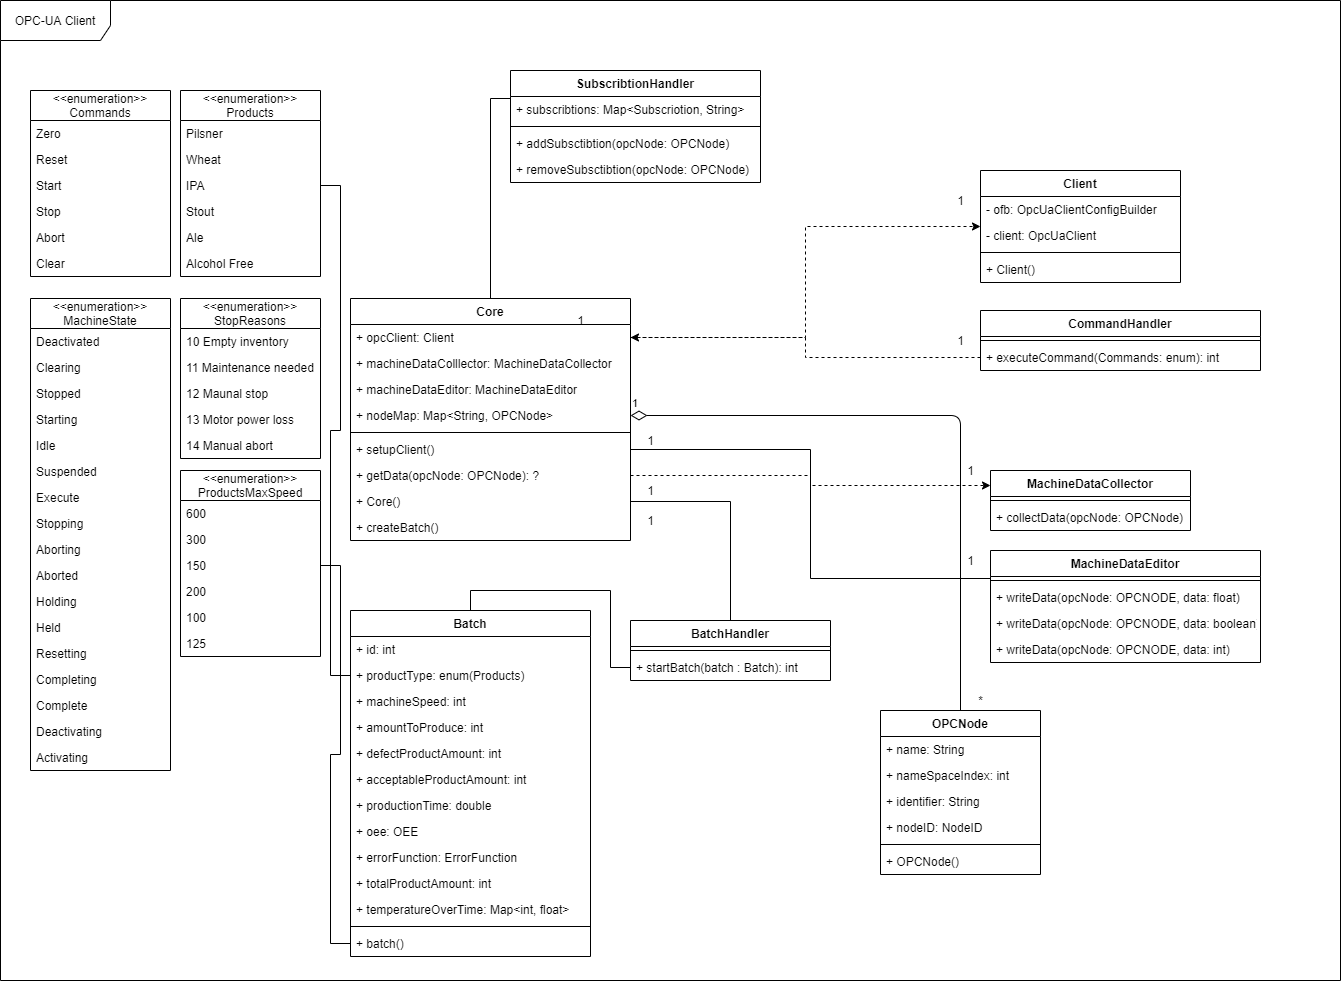
\includegraphics[scale=0.3]{images/diagrams/updated_UML_Class_Diagram.drawio.png}
\caption{Updated UML Class Diagram}
\label{figure:updated_UML_class_diagram} 
\end{figure}


The updated UML class diagram illustrates the current system idea based on the 
analysis up to this point of the project. Although this diagram only shows the 
OPC-UA client it still gives a good idea of how this part of the system is going
to be, once implemented. \\

By using the diagram in implementation, the process gets a solid skeleton to 
expand upon. The classes in the diagram have a chance of not being implemented 
if it is discovered there is no need for them. However, some of them are 
essential for the structure and will most likely not be discarded but changed to 
adhere to the program.